\documentclass[a4paper]{jpconf}

%%%%%%%%%%%%%%%%%%%%%%%
\usepackage{graphicx}
\usepackage{caption}
\usepackage{subcaption}
\captionsetup{compatibility=false}
\usepackage{amsmath}
\usepackage{amssymb}
\usepackage{xcolor}
\usepackage{appendix}
\usepackage{mwe}
\usepackage{mathtools}
\setlength\parindent{0pt}
%%%%%%%%%%%%%%%%%%%%%%%

% Ya quiero terminar este paper

\begin{document}
\title{Analysis of market efficiency based on short term price trends in daily stock-market index data}

\author{H.R Olivares-S\'anchez$^1$, E Scalas$^2$,  A.R. Hern\'andez-Montoya$^3$, C.M. Rodr\'{\i}guez-Mart\'{\i}nez$^3$}

\address{$^1$Facultad de F\'{\i}sica. Universidad Veracruzana, Apdo. Postal 475. Xalapa, Veracruz. M\'{e}xico.}

\address{$^2$Department of Economy, Sussex University,
Universit\`a del Piemonte Orientale ``Amedeo Avogadro'', Viale T. Michel 11, 15121 Alessandria, Italy. BCAM-Basque Center for Applied Mathematics, Alameda de Mazarredo 14, 48009 Bilbao, Basque Contry, Spain.}

\address{$^3$Centro de Investigaci\'on en Inteligencia Artificial. Universidad Veracruzana. Sebasti\'an Camacho 5, Xalapa Veracruz 91000, M\'exico. Tel/Fax: 52-228-8172957/8172855.}


\ead{hectorolivares100@gmail.com, alhernandez@uv.mx, fis.carlosmanuel@gmail.com}

\begin{abstract}
In financial time series there are periods in which the value increases or decreases monotonically. We call those periods {\it elemental trends} and study the probability distribution of their duration for the indices DJIA, NASDAQ, IPC and Nikkei 225. It is found that the trend duration distribution often differs from the one expected under no memory. The expected and observed distributions are compared by means of the Anderson-Darling test.
\end{abstract}

\section{Introduction}
\label{intro}
One of the goals of financial-market analysis is to predict the future movements of prices and financial indices. In order to achieve this goal, a huge variety of methods to forecast markets behavior were developed, ranging from complex mathematical models even to astrological pseudo-scientific techniques. An approach that has been recently growing in popularity is the statistical analysis of large sets of data, which has become now possible due to the increasing availability of computer power and high quality data sets. This approach has benefited from the contributions not only from economists, but also from many physicists and mathematicians who have applied methods and ideas of probability theory and statistical physics to finance. A set of nontrivial statistical properties of historical data was observed and classified as ``stylized facts'' \cite{Rama}, which are expected to provide a better insight on markets structure and behavior.

When observing the time series of the prices of an asset on a chart, it is common to see ``trends'' in which most of the values are greater (or smaller) than the previous ones. These trends are very popular within the so called {\it technical analysis}. Trends as those studied by technical analysis can be seen as composed by smaller elemental trends, periods in which the value increases or decreases monotonically. These kind of trends are the ones that will be studied in the present work. Among other things, technical analysts seek patterns in the charts of financial data, that are believed to be indicators of changes in the trend direction. The effectiveness of technical analysis is disputed and put at a stake by what is known as the Efficient Market Hypothesis. Before going further, it is necessary to give some definitions. In Subsections \ref{def}, \ref{efficient} and \ref{stylized} of this introduction these definitions and other useful information will be presented. In Section \ref{model}, a model for the distribution of trends durations will be developed from the efficient market hypothesis. Section \ref{methodology} will explain how the data were analyzed and section \ref{discussion} provides an interpretation of the analysis.
\subsection{Definitions} 
\label{def}
Let $S(t)$ be the price of an asset or an index value at time $t$ and $X(t) = \log{S(t)}$ its logarithm. The log-return at time $t$ is defined as:
\begin{equation}
r(t,\Delta{t}) = X(t + \Delta{t}) - X(t)
\end{equation}
for a given time sampling scale $\Delta{t}$. If the price variation is small, the log-return is a good approximation of the return
\begin{equation}
R(t,\Delta t) = \frac{S(t+\Delta t) - S(t)}{S(t)}.
\end{equation}
In this paper, we consider $\Delta t$ equal to 1 day and we use the values of the indices corresponding to the close value further in the investigated markets. More details on the data set will be given in section \ref{methodology}.

An {\it elemental trend} of duration $k$ will be defined here as a subseries of $k+1$ values within the series $S(t)$ in which every value is greater (for an uptrend) or smaller or equal (for a downtrend) than the preceding one (Figure \ref{fig:trends}). The aim of this work is to study with a statistical approach the kind of short term trends defined above.

\begin{figure}
\begin{center}
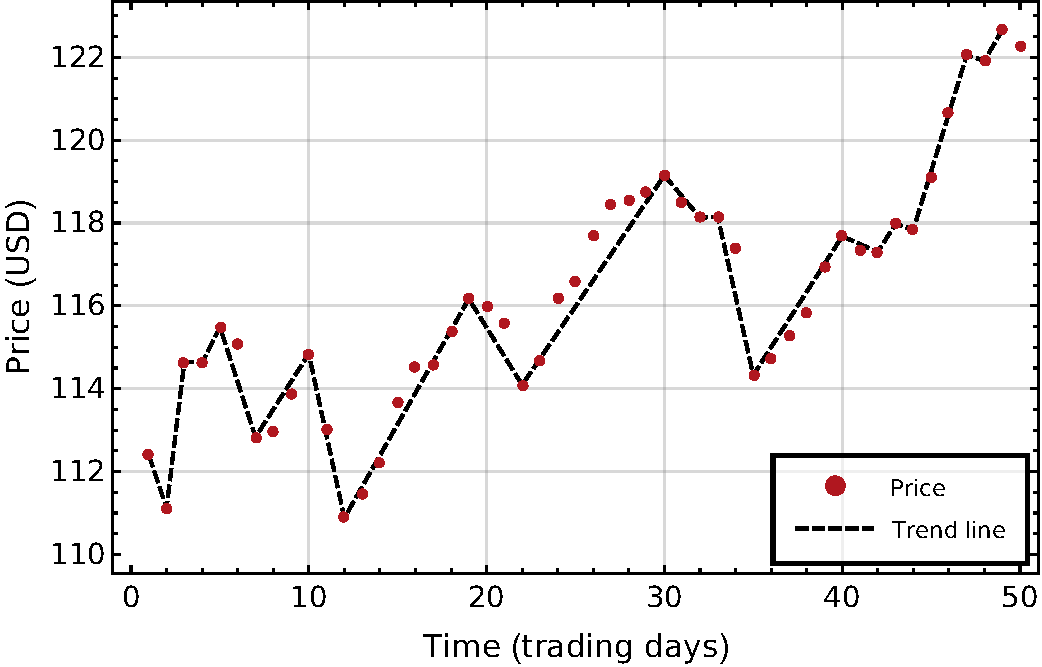
\includegraphics[width=0.45\textwidth]{img/TrendReturnsVisual.pdf}
\end{center}
\caption{\small \label{fig:trends}The line segments join the starting and ending points of each elemental trend for prices of the DJIA. Time period from Oct/30/1978 to Jan/09/1979.}
\end{figure}


\subsection{The Efficient Market Hypothesis}
\label{efficient}
The Efficient Market Hypothesis (EMH) claims that the market quickly finds the rational price for a traded asset \cite{Mantegna}. The most important consequence of this hypothesis was shown by P. Samuelson \cite{Samuelson 2} and it is the fact that the best forecast for the future price of an asset is its present price.
\begin{equation}
\label{emh1}
\mathbb{E}(S(t+\Delta t)|\mathcal{F}_t ) = S(t),
\end{equation} 
where $\mathbb{E}(\cdot|\mathcal{F}_t)$ is the conditional expectation with respect to the filtration $\mathcal{F}_t$, namely with respect to the known history up to time $t$. Indeed, it is easy to derive the EMH from a simple no-arbitrage argument. Suppose we have two assets, a risky one, with price $S(t)$ and a risk-free one giving a constant interest rate $r_F$. To avoid arbitrage, one has to require that the expected return of the risky asset is equal to the risk-free interest rate, that is
\begin{equation}
\mathbb{E} (R(t, \Delta t)|\mathcal{F}_t) = r_F;
\end{equation}
the latter equation immediately yields, for non vanishing $S(t)$,
\begin{equation}
\label{emh2}
\mathbb{E}(S(t+\Delta t)|\mathcal{F}_t ) = (1+r_F) S(t),
\end{equation}
which reduces to \eqref{emh1} for $r_F = 0$. Equations \eqref{emh1} and
\eqref{emh2}, jointly with the integrability of the process $S(t)$, are known as martingale and sub-martingale conditions (remember that under normal conditions $r_F \geq 0$), respectively.

The EMH would invalidate the attempts of technical analysis to predict future prices or trends; in fact, in Samuelson's words, ``there is no way of making an expected profit by extrapolating past changes in the futures price, by chart or any esoteric devices of magic or mathematics'' \cite{Samuelson 2} as the best forecast of the future price would be the current price.

\subsection{Stylized facts}
\label{stylized}
As mentioned before, financial time series share some nontrivial statistical properties called stylized facts. Although those properties are often formulated qualitatively, they are so constraining that it is difficult to reproduce all of them by means of a stochastic process\cite{Rama}. As a matter of fact, none of the market models, including analytical models, Monte Carlo simulations and multi-agent based models, created before 1990, when awareness of such regularities gradually started to appear, could reproduce all of these stylized facts \cite{Lux}. As an interesting issue, some studies suggest that stylized facts appear not only in financial time series, but also in other complex systems such as Conway's Game of Life \cite{Hernandez}. To fix the ideas, some of the stylized facts, taken from reference \cite{Rama}, are listed below:

\begin{description}
\item[Absence of linear autocorrelations:] Autocorrelations of returns are often negligible, except for very small time scales, depending on the market and on the time horizon.
\item[Heavy tails:] The return distribution is leptokurtic and some authors claim that the tails decay as a power-law.
\item[Gain-loss asymmetry:] Large downward jumps in stock prices and stock index values are observed, but not equally large upward movements. (In exchange rates there is a higher symmetry in up/down movements).
\item[Volatility clustering:] High volatility events do cluster in time.
\end{description}

\section{An `Efficient Market' model for the duration distribution}
\label{model}
Among all the possible martingale or sub-martingale models that can describe price fluctuations, the geometric random walk is the simplest one. A geometric random walk is just a product of independent and identically distributed positive random variables. If the expected value of these variables is $1$, then the geometric random walk is a martingale; otherwise, if the expected value is larger than $1$, the geometric random walk is a submartingale. However, the geometric random walk hypothesis is neither necessary nor sufficient for an efficient market, as shown by many authors among whom Leroy \cite{leroy}, Lucas \cite{lucas} and Lo and Mackinlay \cite{lo}. To understand this point, it is enough to consider Equation \eqref{emh2} allowing for any martingale model.

At each step of a series of index values, there are two possible outcomes: the index either increases or does not increase. In an efficient market, the expected future price depends only on information about the current price, not on its previous history. Therefore, it should be impossible to predict the expected direction of a future price change given the history of the price process. In formula, from Equation \eqref{emh1} (after discounting for the risk-free rate), we have\begin{equation}
\label{expectedincrement}
\mathbb{E}(S(t+\Delta t) - S(t)|\mathcal{F}_t)= 0;
\end{equation}
if we consider the sign of the price change $Y(t,\Delta t)=\mathrm{sign}(S(t+\Delta t)-S(t))$, which coincides with the sign of returns, we accordingly have
\begin{equation}
\label{expectedsign}
\mathbb{E}(Y(t,\Delta t))=0.
\end{equation}

If the price follows a geometric random walk, then the series of price-change signs can be modeled as a Bernoulli process. This process could be biased to take the presence of a risk-free interest rate into account. To be more specific, let us consider a log-normal geometric random walk and let us use the assumption $\Delta t =1$. Let $S_0$ be the initial price. The price at time $t$ will be given by
\begin{equation}
S(t)=S_0 \prod_{i=1}^t Q_i
\end{equation}
where $Q_i$ are independent and identically distributed random variables following a log-normal distribution with parameters $\mu$ and $\sigma$. These two parameters come from the corresponding normal distribution for log-returns. As a direct consequence of the EMH in the form \eqref{emh2}, we have
\begin{equation}
\mathbb{E} (Q) = 1 + r_F,
\end{equation}
and for a log-normal distributed random variable, we have also
\begin{equation}
\mathbb{E}(Q) = \mathrm{e}^\mu \mathrm{e}^{\sigma^2/2}.
\end{equation}
This leads to a dependence between the two parameters
\begin{equation}
\sigma = \sqrt{2\left(\log(1+r_f)-\mu \right)}
\end{equation}
Starting from the cumulative distribution function for a log-normal random variable
\begin{equation}
F_Q(u)=\mathbb{P}(Q \leq u) = \frac{1}{2} + \frac{1}{2} \mathrm{erf}\left(
\frac{\log(u) -\mu}{\sqrt{2 \sigma^2}} \right),
\end{equation}
the probability of a negative sign would be given by
\begin{equation}
q=F_Q(1)=\mathbb{P}(Q \leq 1)=\frac{1}{2} + \frac{1}{2} \mathrm{erf}\left(
\frac{- \mu}{\sqrt{4(\log(1+r_f)-\mu)}} \right),
\end{equation}
which yields $q = 0.5 \pm 0.05$ for typical markets (see figure \ref{fig:qvalue}).

\begin{figure}[h!tb]
	\centering
        \begin{subfigure}[b]{0.45\textwidth}
            \centering
            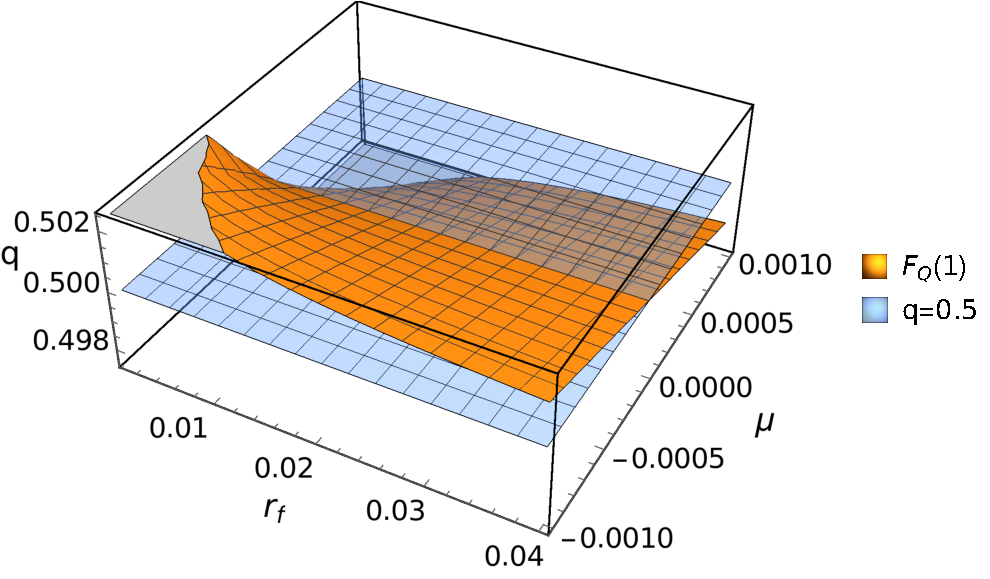
\includegraphics[width=\textwidth]{img/model_q}
            \caption[]{\small Probability of negative return given the risk-free interest rate $r_f$ and mean $\mu$. The $\mu$ parameter can be estimated from the return time series $Q_i$, and $r_f$ is estimated from a reference asset that depends on the market being studied. Intersection with $q=0.5$ is also shown.}    
            \label{fig:model_q}
        \end{subfigure}
        \quad
        \begin{subfigure}[b]{0.45\textwidth}  
            \centering 
            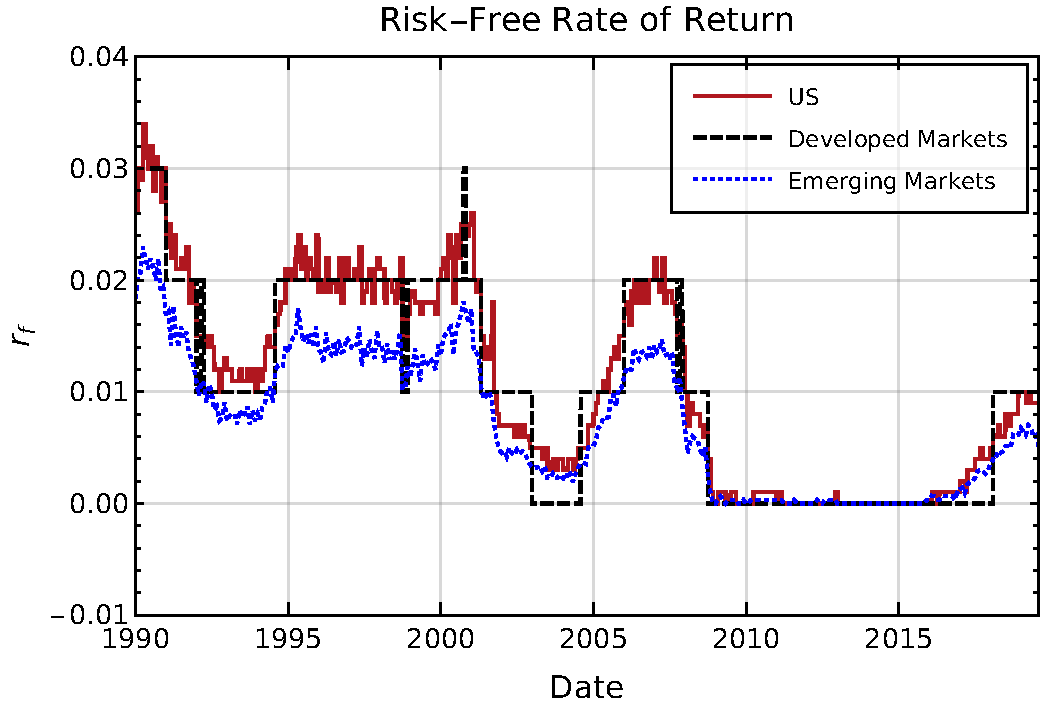
\includegraphics[width=\textwidth]{img/riskfree_rate}
            \caption[]{\small Risk-Free rate of returns $r_f$ for the US market, developed markets and emerging markets \cite{French}. For the period ranging from $1978$ to $2018$ the risk-free rate oscillates between the interval $[0, 0.061)$.}
            \label{fig:rf}
      
        \end{subfigure}
        \caption{\small For a tipical time series of $Q_i$ the parameter $\mu$ is close to zero oscillating on a small interval ranging from $-0.001$ to $0.001$. The risk-free rate of return $r_f$ oscillates between the interval $[0, 0.061)$. For these values the probability of a negative return is $q = 0.5 \pm 0.05$.} 
	\label{fig:qvalue}
\end{figure}

It becomes natural to use the biased Bernoulli process as the null hypothesis for the time series of signs \cite{scalasold}. It is well known that the distribution of the number $k$ of failures needed to get one success for a Bernoulli process with success probability $p=1-q$ is the geometric distribution ${\cal{G}}(p)$; the number of failures $N$ is given by
\begin{equation}
P(k)=\mathbb{P}(N=k) = p(1 - p)^{k} = pq^{k}.
\end{equation}
The duration of a elemental downward trend in daily data is the number of days before the price increases, so the distribution of such trend durations should follow a geometric distribution. An identical argument applies to the duration of a upward trend. Such sequences of identical outcomes are also known as {\em runs} or {\em clumps} in the mathematical literature.

\section{Methodology}
\label{methodology}
\subsection{Data}
Four indices were analyzed, namely Dow Jones Industrial Average (DJIA), NASDAQ Composite, the Mexican \'Indice de Precios y Cotizaciones (IPC) and Nikkei 225 during the period 30 October 1978 - 26 September 2019. The data was obtained from Yahoo Finance.

\subsection{Building the sample}
For each series of index values, several time windows of 504 trading days (which represent two trading years in average) were created, each one shifted forward by one trading day with respect to the previous one. This procedure resulted in 4830 time windows for the DJIA, 4216 for the NASDAQ, 3901 for the IPC and 4584 for the Nikkei. For every sample in the time windows, the number of days at time $t$ before every sign change $T_d(t)$ (defined as the trend duration) is measured. For instance, given the sequence $-$ $ - + + + + + $ $-$, the recorded times will be $T_d = (2,5,1)$.

Two histograms were built for each market measuring $T_d$ on the whole sample without time windows. One for upward trends and the other one for downward trends. Examples of both uptrend and downtrend histograms for different time windows are shown in Figure \ref{fig:oneGT}.


\subsection{The Anderson-Darling goodness of fit test}
In order to compare the observed and expected distributions of  trend durations, the Anderson-Darling test described in reference \cite{Anderson} was used. The Anderson-Darling test was found to be the most suitable for this purpose because it places more weight on the tails of a distribution than other goodness of fit tests.

Two separate tests were applied. The first is a test of whether the observed data is drawn from a distribution belonging to a parametric family $\mathcal{G}(p)$. This tell us whether the price fluctuations can be modelled as a Bernoulli process. The second is a test of whether the observed data comes from a geometric distribution with $p = 0.5$. Based on the model outlined in section \ref{model} we interpret a rejection of this null hypothesis as evidence that the market is not efficient.

For a more complete discussion on Anderson-Darling Methodology see appendix \ref{apendice}.

\section{Discussion}
\label{discussion}

\begin{figure}
\begin{center}
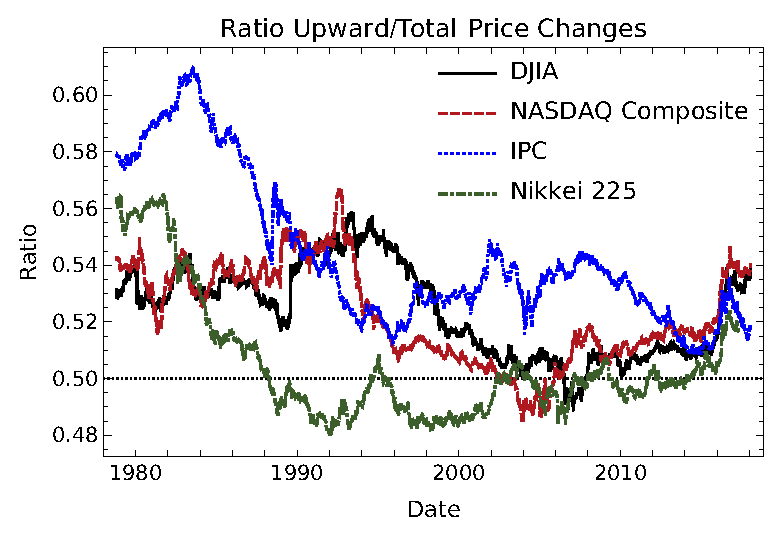
\includegraphics[width=0.45\textwidth]{img/sign_ratios}
\end{center}
\caption{\small \label{fig:simetria}Ratio of upward to total price changes in daily data, plotted against time for the interval from 1978-10-30 to 2019-09-26, calculated over a time window of 504 trading days.}
\end{figure}

In Figure \ref{fig:simetria}, the ratio of the upward to total price changes in daily data is plotted against time for the years 1978 - 2019. This ratio is calculated over a time window of 504 trading days. It can be seen that variations are greater than those expected for the same time windows in a Bernoulli process with parameter $p = 1/2$ ($\pm{0.05}$). Plots in figure \ref{fig:oneGT} show the distribution of trend durations corresponding to different indices. Figure \ref{fig:PiValuesAD} display the $p$-values of the Anderson-Darling statistic for different periods. In order to avoid confusion between the parameter of the geometric distribution and the $p$-values for the distribution of $A^{2}_{n}$, the latter will be referred to as $\pi$-values. The meaning of $\pi$-values is the probability of obtaining a value of $A^{2}_{n}$ at least as big as the one that was really obtained, given that the probability distribution is actually geometric.

%Las cuatro figuras juntas de la prueba paramétrica
\begin{figure}[h!tb]
	\centering
        \begin{subfigure}[b]{0.45\textwidth}
            \centering
            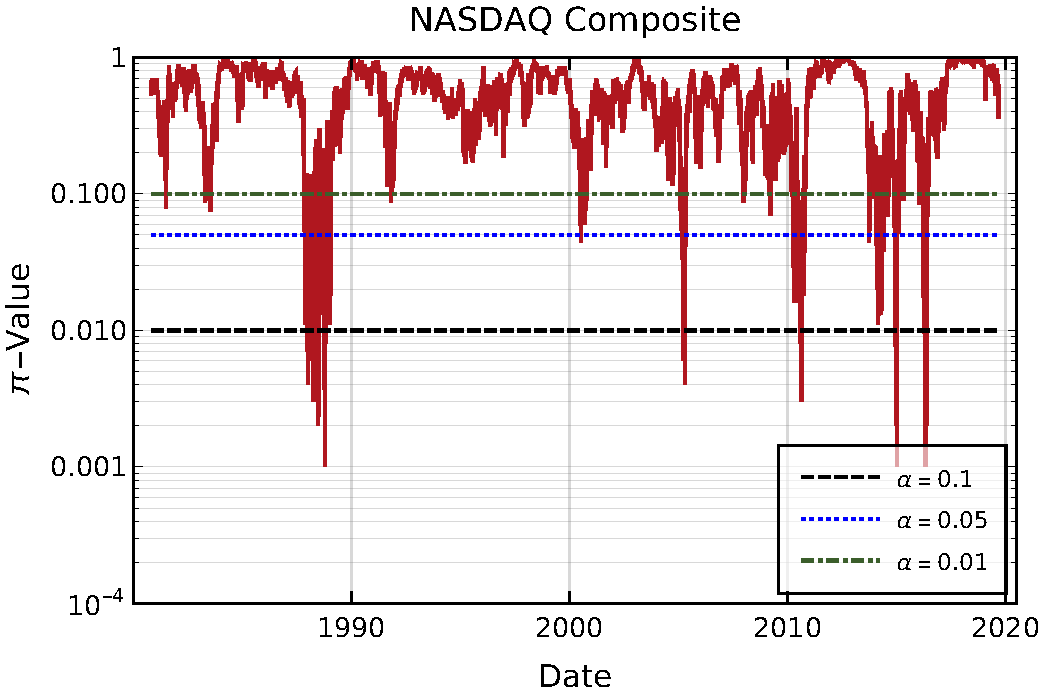
\includegraphics[width=\textwidth]{img/pvalores_family_NASDAQ.pdf}
            \caption[]{}    
            \label{fig:nasdaq_fam}
        \end{subfigure}
        \quad
        \begin{subfigure}[b]{0.45\textwidth}  
            \centering 
            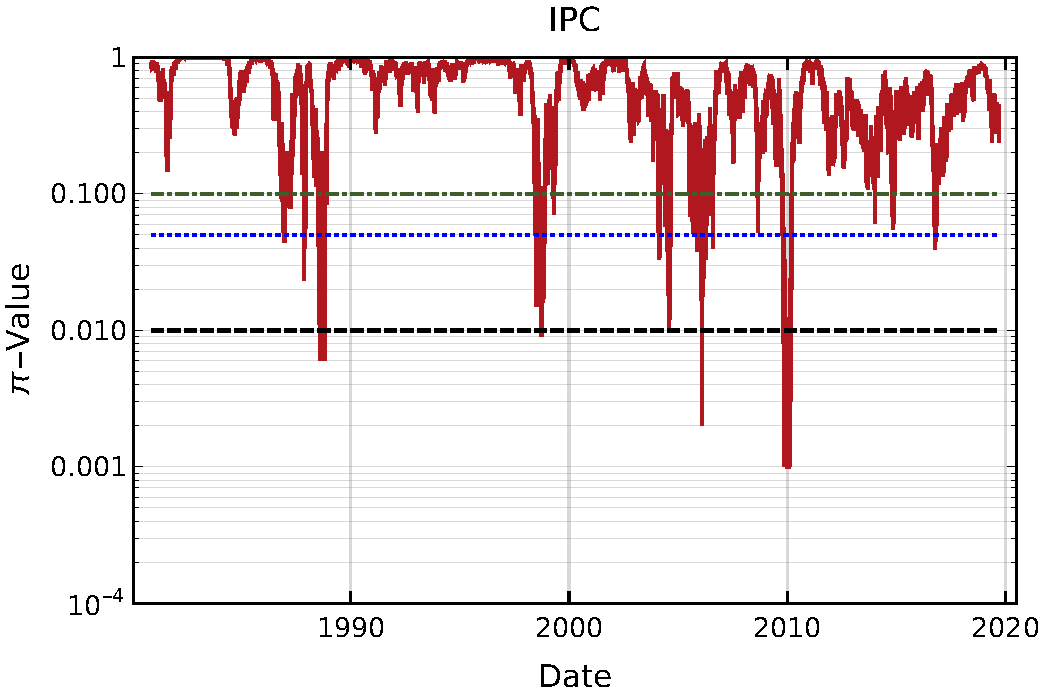
\includegraphics[width=\textwidth]{img/pvalores_family_IPC.pdf}
            \caption[]{}     
            \label{fig:ipc_fam}
        \end{subfigure}
        \vskip\baselineskip
        \begin{subfigure}[b]{0.45\textwidth}   
            \centering 
            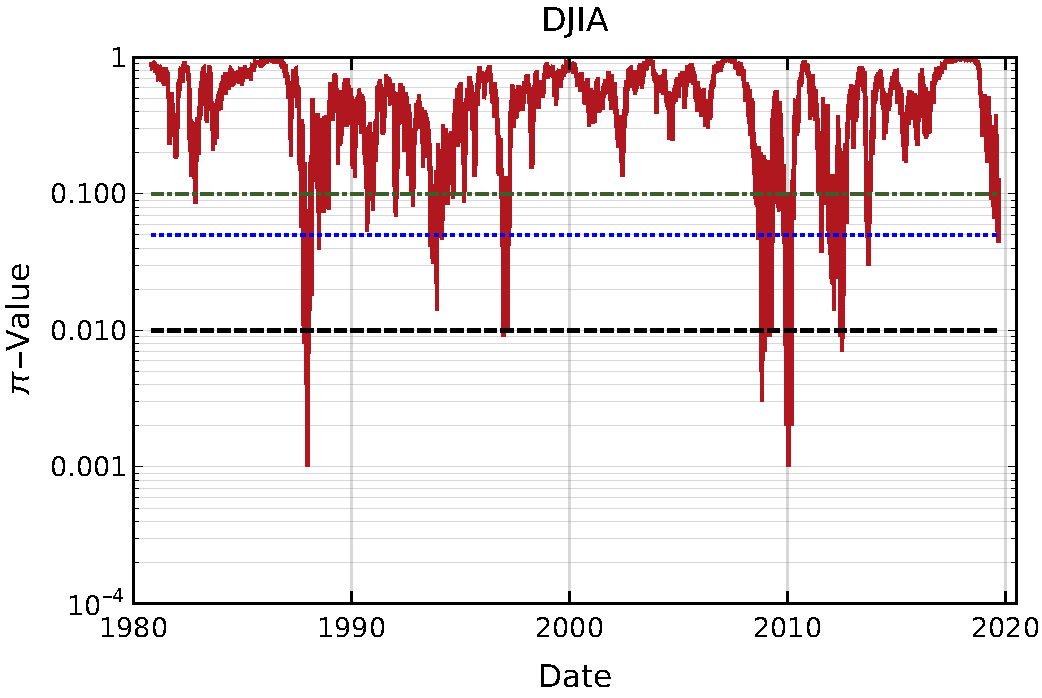
\includegraphics[width=\textwidth]{img/pvalores_family_DJIA.pdf}
            \caption[]{}      
            \label{fig:dji_fam}
        \end{subfigure}
        \quad
        \begin{subfigure}[b]{0.45\textwidth}   
            \centering 
            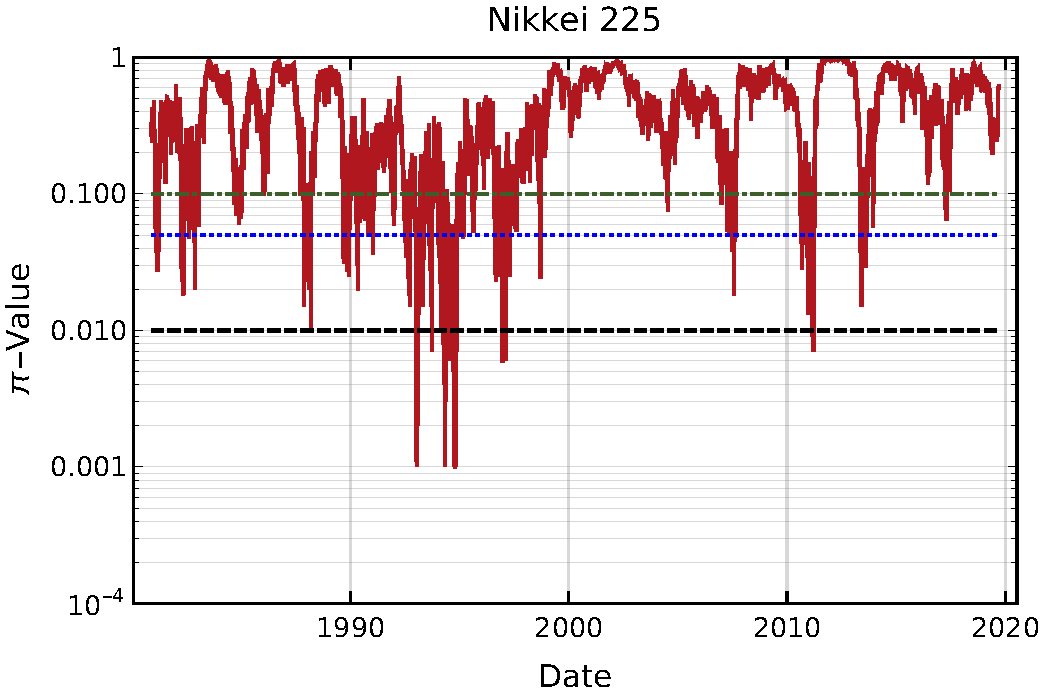
\includegraphics[width=\textwidth]{img/pvalores_family_Nikkei.pdf}
            \caption[]{}      
            \label{fig:nikkei_fam}
        \end{subfigure}
        \caption{\small \ref{fig:nasdaq}: $\pi$-values of the parametric family Anderson-Darling statistic for the studied markets.} 
	\label{fig:PiValuesADFam}
\end{figure}

\begin{figure}
\begin{center}
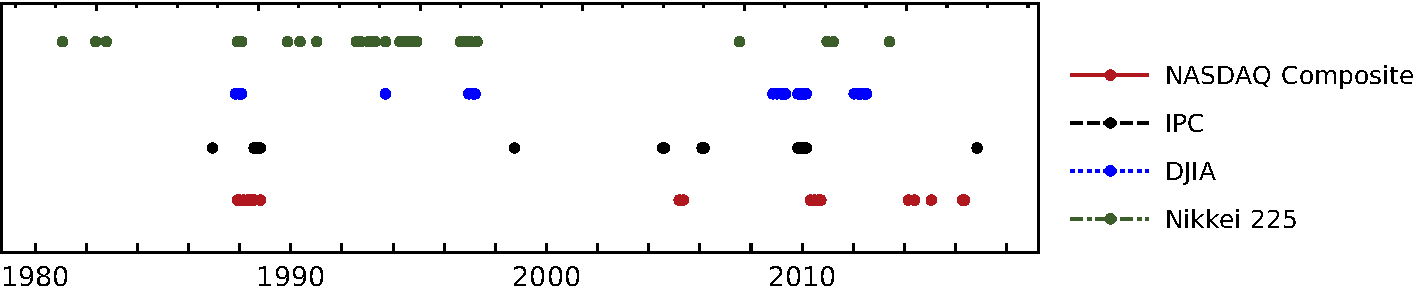
\includegraphics[width=0.70\textwidth]{img/not_geom_dates}
\end{center}
\caption{\small \label{fig:not_geom}Dates where events from figure \ref{fig:PiValuesADFam} have a $\pi$-value below the $\alpha = 0.05$ confidence level.}
\end{figure}

For the parametric family test in figure \ref{fig:PiValuesADFam}, it was observed that the assumption of a Bernoulli process for price directions holds reasonably well most of the time, except for sporadic deviations that are usually present around extreme market movements like a financial crisis.

%Las cuatro figuras juntas, con incisos:
\begin{figure}[h!tb]
	\centering
        \begin{subfigure}[b]{0.45\textwidth}
            \centering
            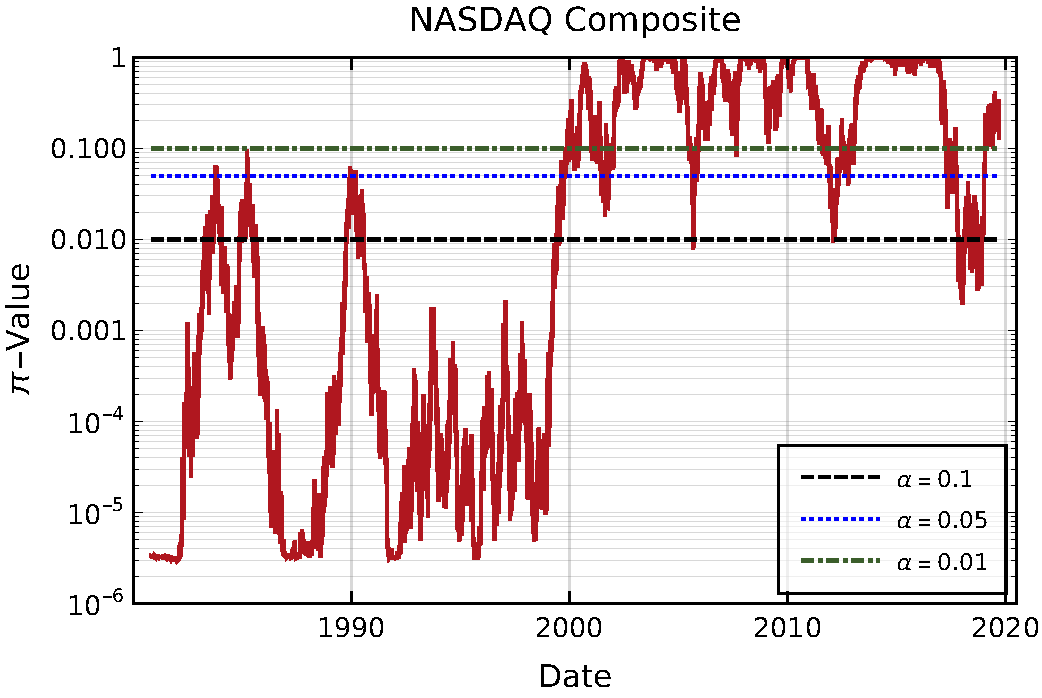
\includegraphics[width=\textwidth]{img/pvalores_NASDAQ.pdf}
            \caption[]{}    
            \label{fig:nasdaq}
        \end{subfigure}
        \quad
        \begin{subfigure}[b]{0.45\textwidth}  
            \centering 
            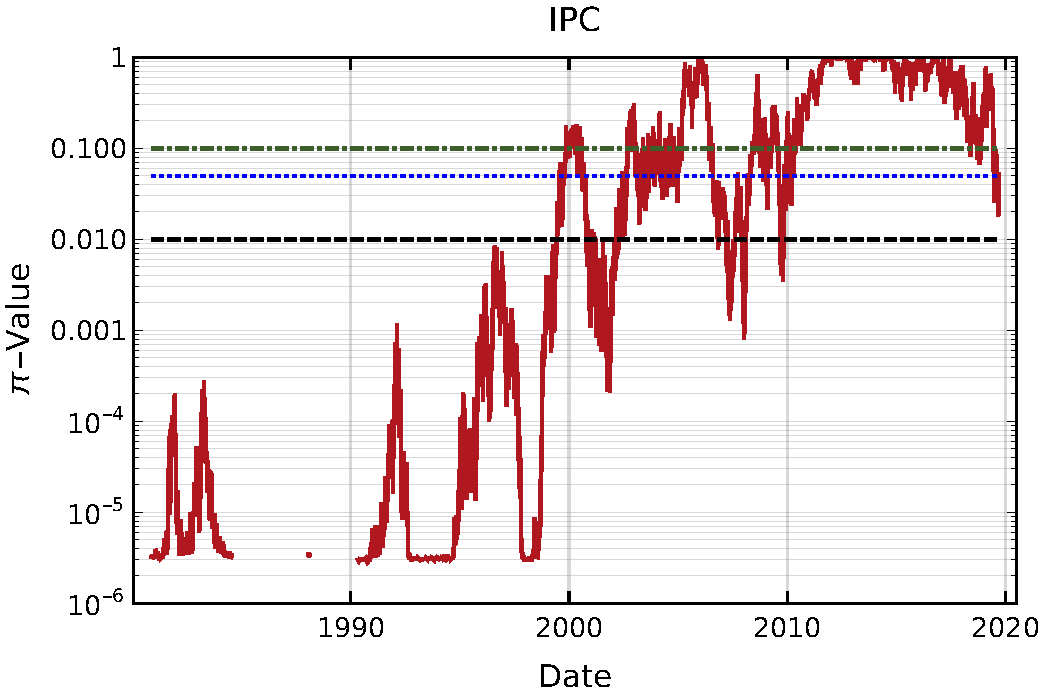
\includegraphics[width=\textwidth]{img/pvalores_IPC.pdf}
            \caption[]{}     
            \label{fig:ipc}
        \end{subfigure}
        \vskip\baselineskip
        \begin{subfigure}[b]{0.45\textwidth}   
            \centering 
            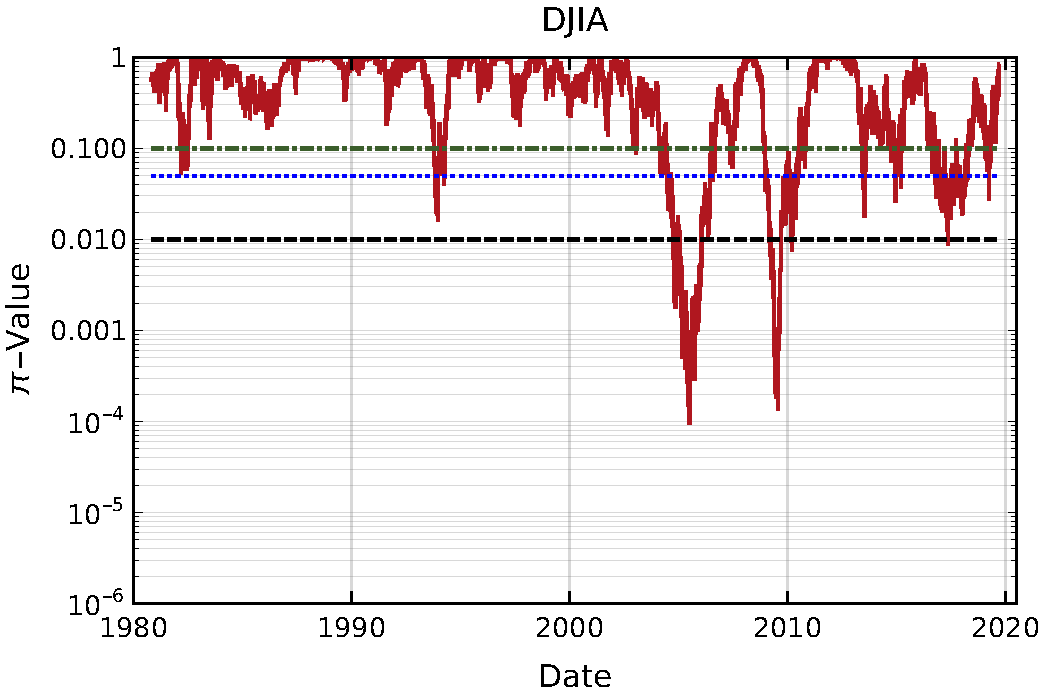
\includegraphics[width=\textwidth]{img/pvalores_DJIA.pdf}
            \caption[]{}      
            \label{fig:dji}
        \end{subfigure}
        \quad
        \begin{subfigure}[b]{0.45\textwidth}   
            \centering 
            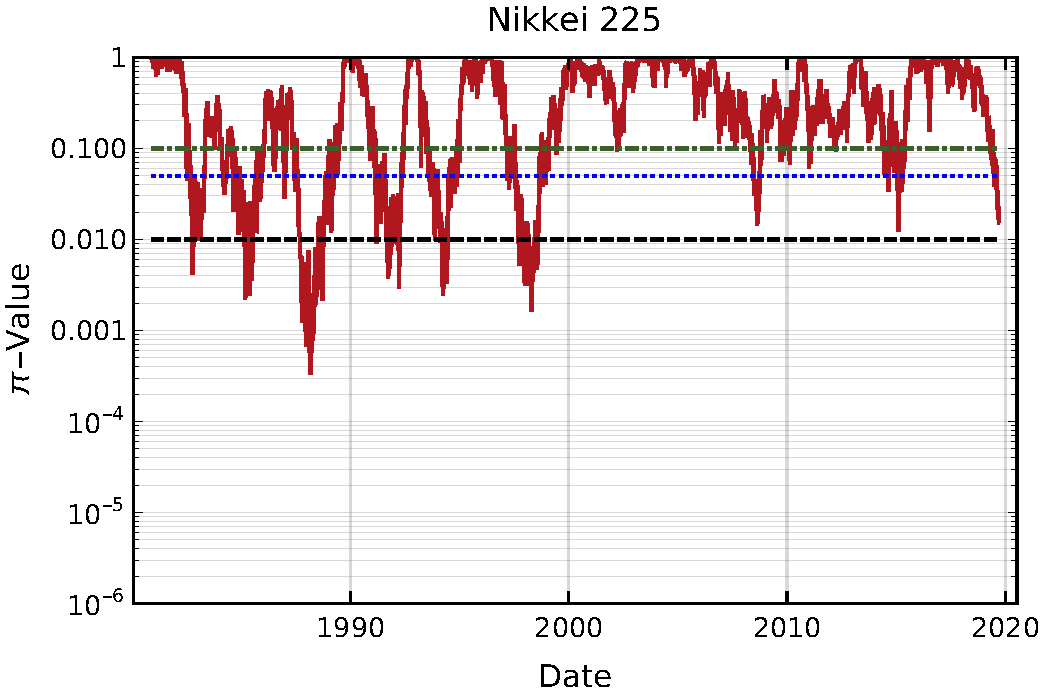
\includegraphics[width=\textwidth]{img/pvalores_Nikkei.pdf}
            \caption[]{}      
            \label{fig:nikkei}
        \end{subfigure}
        \caption{\small \ref{fig:nasdaq}: $\pi$-values of the Anderson-Darling statistic for the NASDAQ plotted against time. As time passes, the data agree better with the geometric distribution $\mathcal{G}(0.5)$; \ref{fig:ipc}: $\pi$-values of the Anderson-Darling statistic for the IPC plotted against time. As for NASDAQ, agreement between data and the geometric distribution increases with time;  \ref{fig:dji}: $\pi$-values of the Anderson-Darling statistic for the DJIA plotted against time. The greatest deviations from the geometric distribution occurred between the years 2000-2011. \ref{fig:nikkei}: $\pi$-values of the Anderson-Darling statistic for the Nikkei plotted against time. The greatest deviations from the geometric distribution occurred between the years 1980-2000.} 
	\label{fig:PiValuesAD}
\end{figure}

\begin{figure}
\begin{center}
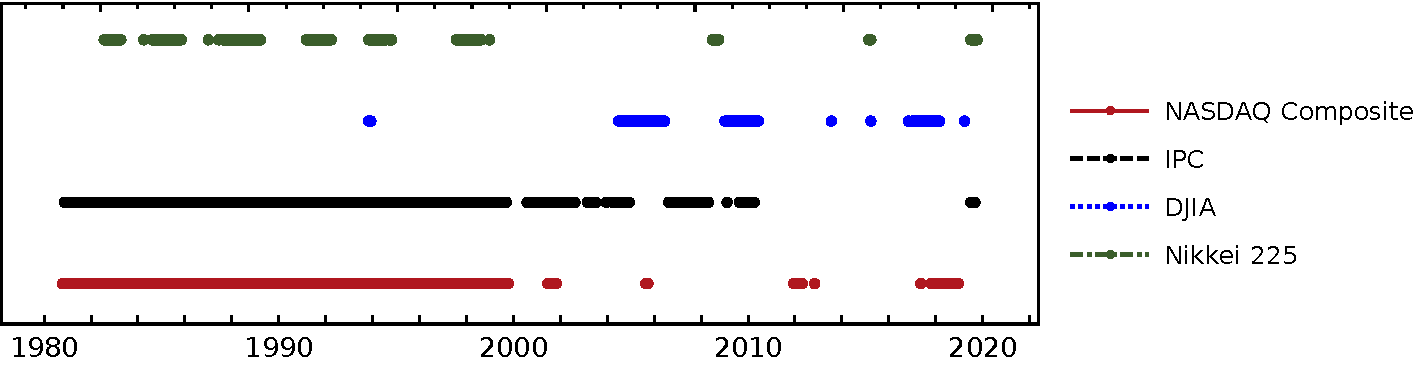
\includegraphics[width=0.70\textwidth]{img/not_eff_dates}
\end{center}
\caption{\small \label{fig:not_geom}Dates where events from figure \ref{fig:PiValuesAD} have a $\pi$-value below the $\alpha = 0.05$ confidence level.}
\end{figure}

% Histogramas de duración de trends
\begin{figure}[h!tb]
	\centering
        \begin{subfigure}[b]{0.45\textwidth}
            \centering
            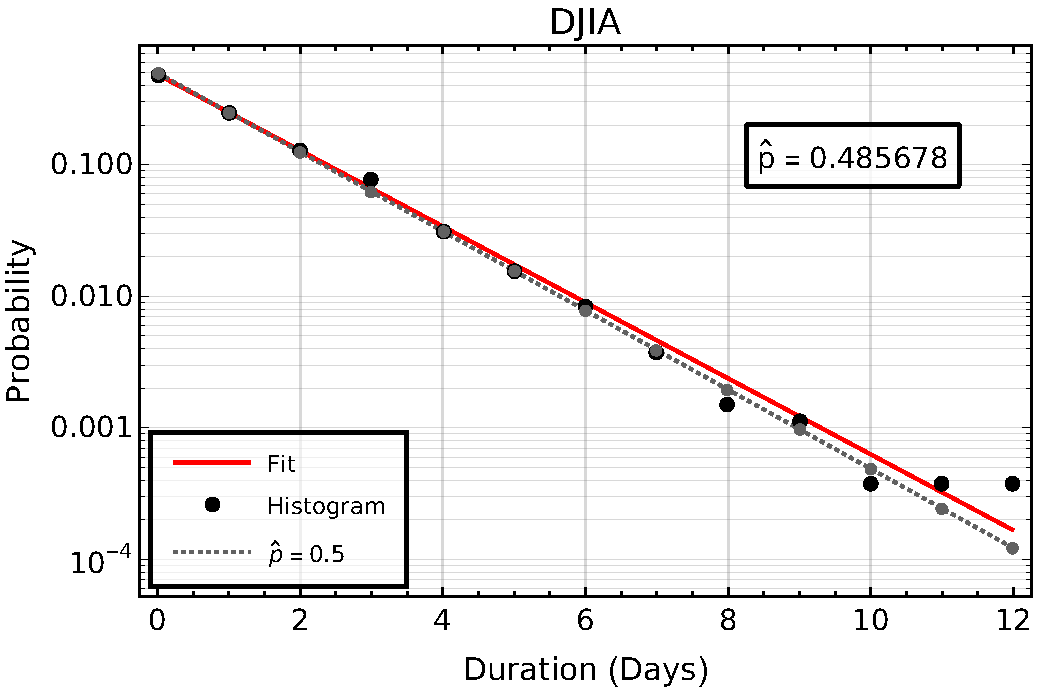
\includegraphics[width=\textwidth]{img/dist_pos_DJIA.pdf}
            \caption[]{}    
        \end{subfigure}
        \quad
        \begin{subfigure}[b]{0.45\textwidth}  
            \centering 
            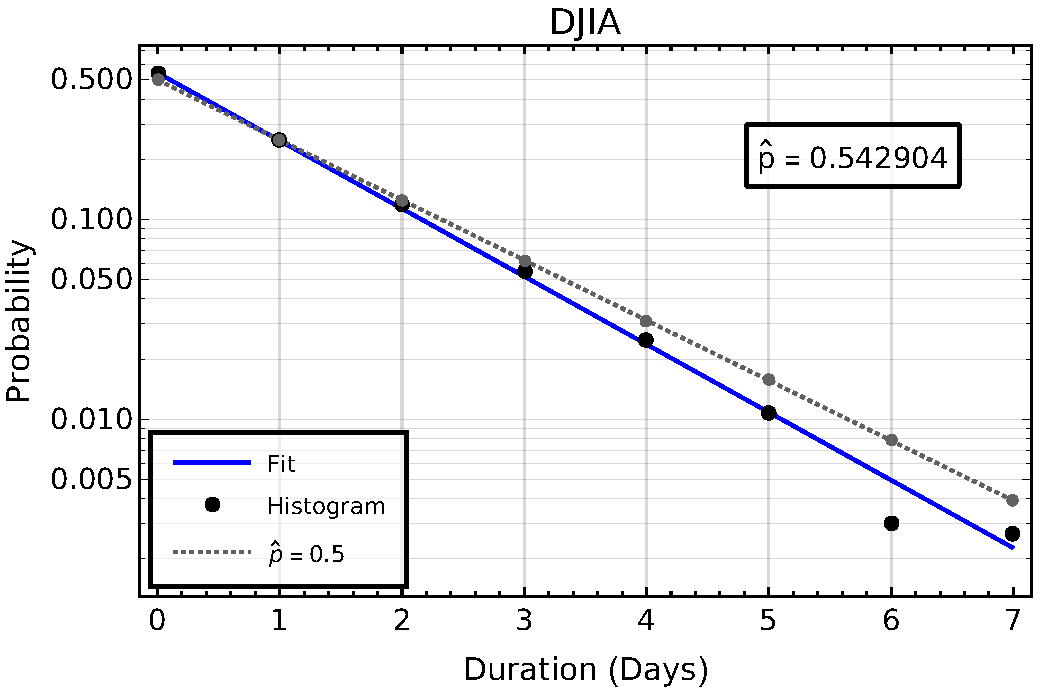
\includegraphics[width=\textwidth]{img/dist_neg_DJIA.pdf}
            \caption[]{}     
        \end{subfigure}
        \vskip\baselineskip
        \begin{subfigure}[b]{0.45\textwidth}   
            \centering 
            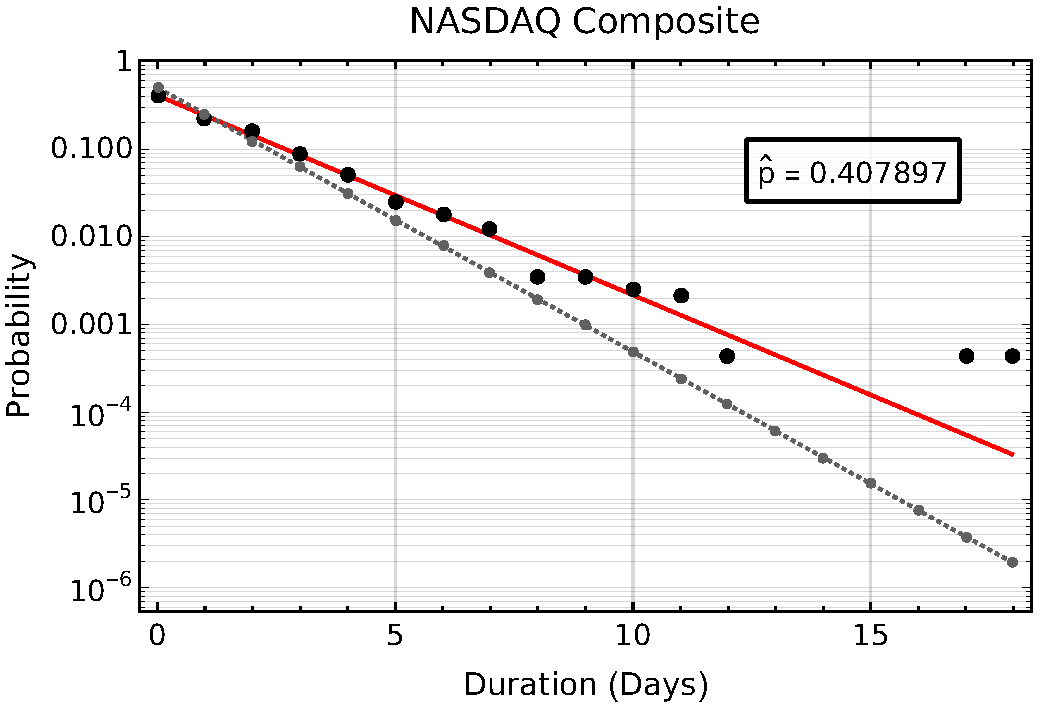
\includegraphics[width=\textwidth]{img/dist_pos_NASDAQ.pdf}
            \caption[]{}      
        \end{subfigure}
        \quad
        \begin{subfigure}[b]{0.45\textwidth}   
            \centering 
            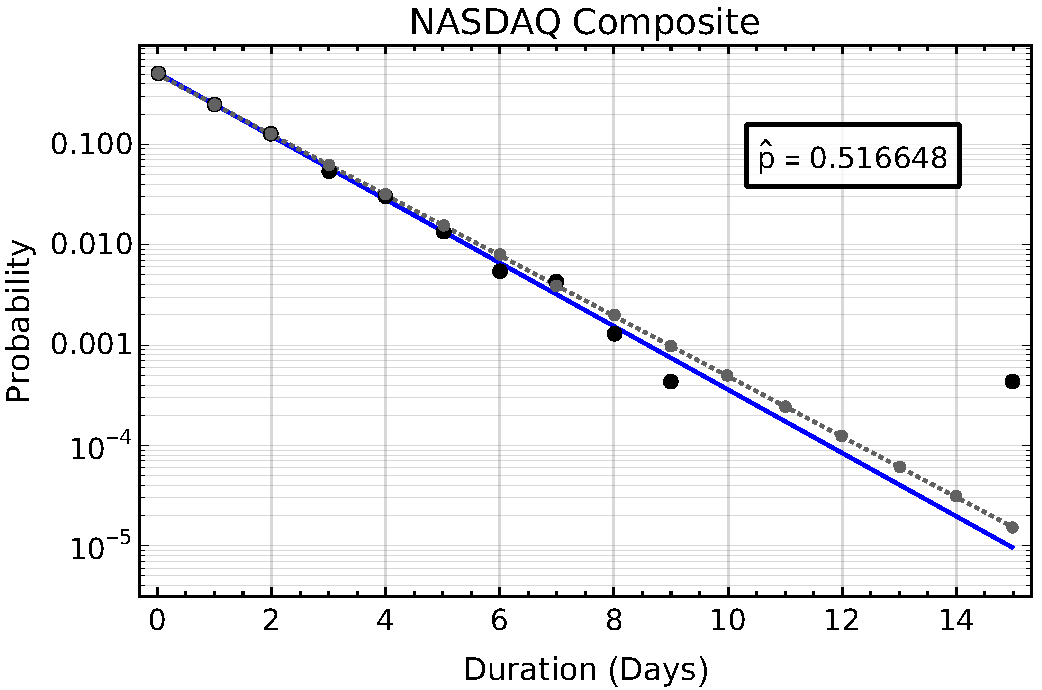
\includegraphics[width=\textwidth]{img/dist_neg_NASDAQ.pdf}
            \caption[]{}      
        \end{subfigure}
        \begin{subfigure}[b]{0.45\textwidth}
            \centering
            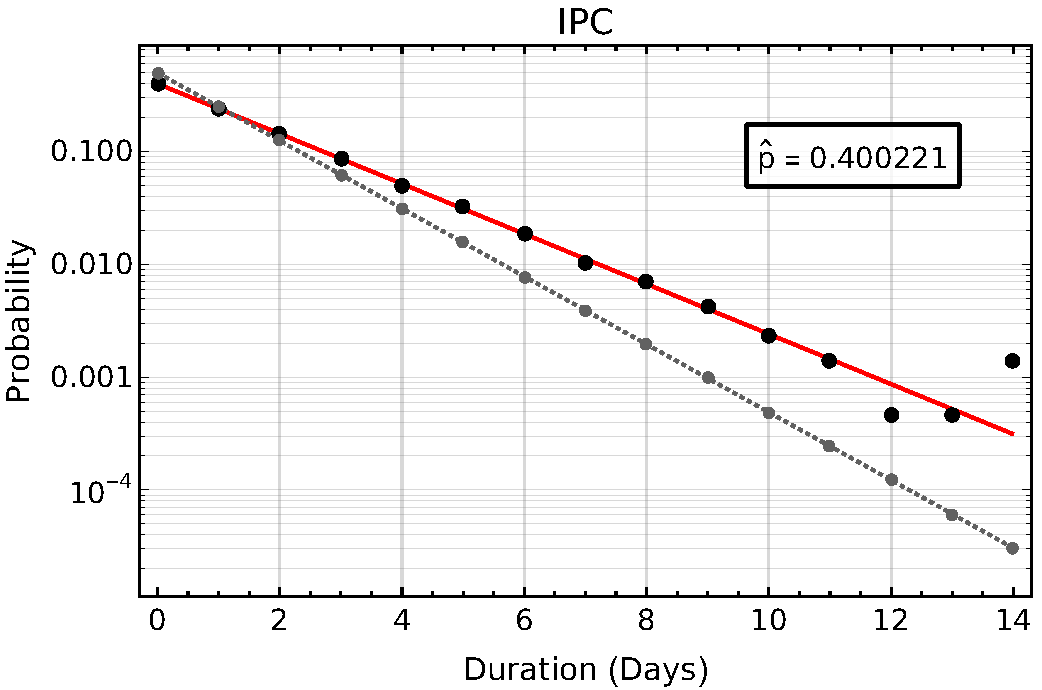
\includegraphics[width=\textwidth]{img/dist_pos_IPC.pdf}
            \caption[]{}    
        \end{subfigure}
        \quad
        \begin{subfigure}[b]{0.45\textwidth}  
            \centering 
            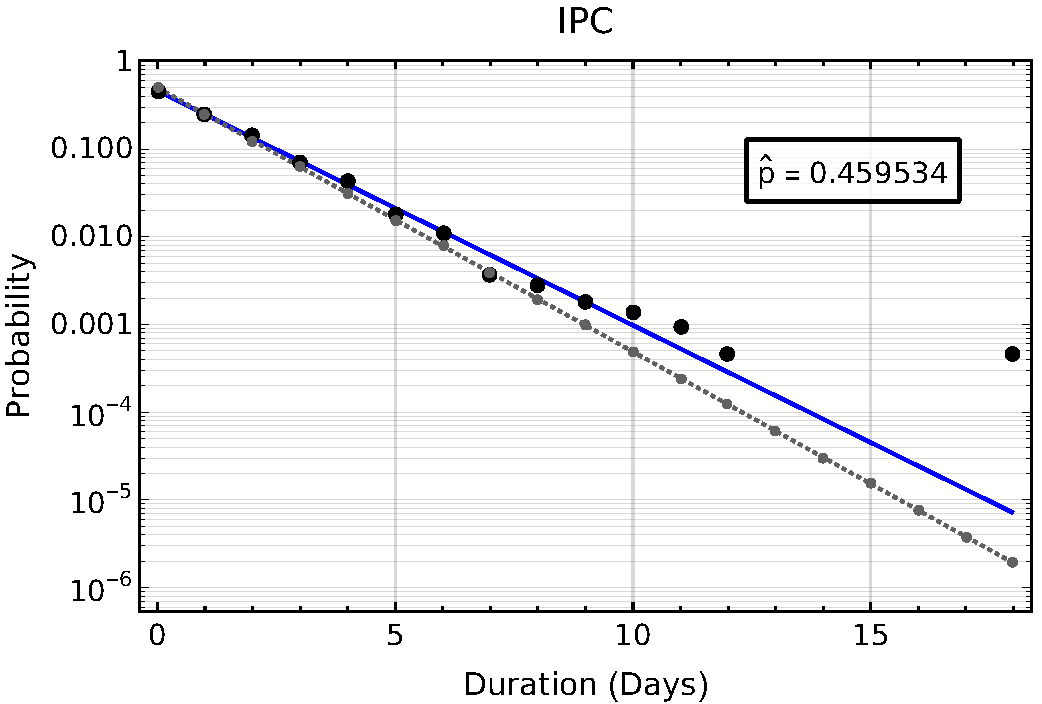
\includegraphics[width=\textwidth]{img/dist_neg_IPC.pdf}
            \caption[]{}     
        \end{subfigure}
        \vskip\baselineskip
        \begin{subfigure}[b]{0.45\textwidth}   
            \centering 
            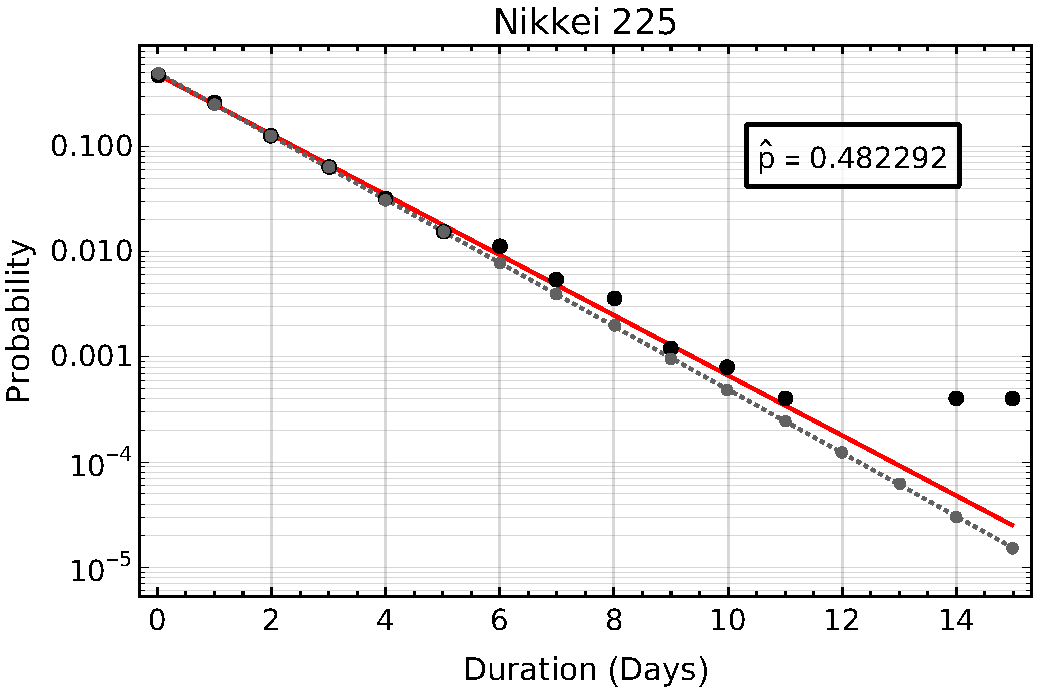
\includegraphics[width=\textwidth]{img/dist_pos_Nikkei.pdf}
            \caption[]{}      
        \end{subfigure}
        \quad
        \begin{subfigure}[b]{0.45\textwidth}   
            \centering 
            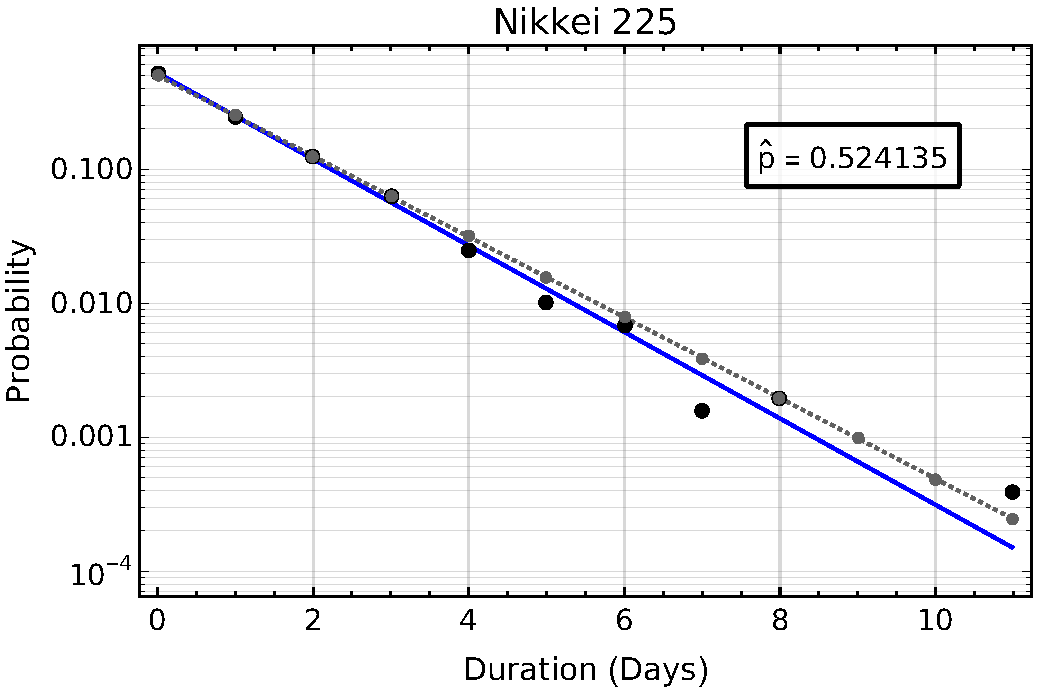
\includegraphics[width=\textwidth]{img/dist_neg_Nikkei.pdf}
            \caption[]{}      
        \end{subfigure}
        \caption{\small Distribution of trend durations $T_d$ for different indices. (a), (c), (e) and (g) present the upward distribution and (b), (d), (f) and (h) the downward distribution. The solid lines are the fitted geometric distributions while the dotted lines are the expected geometric distributions ($p = 0.5$). The parameter $\hat{p}$ is shown on each figure.} 
	\label{fig:oneGT}
\end{figure}


It was observed that as time passes, the direction of price changes for the IPC and the NASDAQ is better described by a geometric distribution following the efficient market hypothesis $\mathcal{G}(0.5)$ (Figures \ref{fig:nasdaq} and \ref{fig:ipc}). Meanwhile the distribution of trend durations for the Dow Jones and Nikkei is generally reasonably well fitted by the geometric distribution. This fact can be interpreted as a possible evidence that the Mexican stock market (that has become public and regulated since 1975) has been increasing its efficiency, as reported by previous research \cite{Achach}. The same claim can be made about the NASDAQ, given that it is also a market of relatively recent creation. In contrast, the Dow Jones Industrial Average index represents a more mature market. However, there is also evidence that the New York Stock Exchange, represented by the Dow Jones, has swiftly increased its efficiency between the beginning of the 1980s and the end of the 1990s \cite{NYSE}. Figure \ref{fig:dji} shows that for the Dow Jones, the greatest deviations from the geometric distribution in the studied period occurred between the years 2000-2011. Figure \ref{fig:nikkei} shows that for the Nikkei, the greatest deviations from the geometric distribution in the studied period occurred between the years 1980-2000.


\section{Conclusions}
The probability distributions for the duration of elemental trends were studied for the market indices Dow Jones Industrial Average (DJIA), NASDAQ Composite, the Mexican \'Indice de Precios y Cotizaciones (IPC) and for the Japanese Nikkei 225. These distributions are expected to be geometric and memoryless according to the discussion in section \ref{model}. The IPC and the NASDAQ present periods in which the memoryless hypothesis must be definitively rejected, while DJIA and Nikkei showed to be fitted reasonably well by geometric distribution with sporadic deviations.

\clearpage

\begin{appendices}
\addappheadtotoc
\appendixpage
  
\section*{The discrete version of the Anderson-Darling goodness of fit test}
\label{apendice}
 %\section{The discrete version of the Anderson-Darling goodness of fit test}

% Why Chi2 is not effective
Determining whether or not a given probability model fits the observed data that it attempts to describe is one of the most important problems of applied statistics. Even though extensive research has been done regarding this problem, most of it deals with continuous distributions. Unfortunately, the studies done for fitting discrete distributions are much less numerous, or at least harder to find.

Discrete distributions, however, are important in many fields as medicine, psychology and engineering. Scientific papers and textbooks often prescribe the chi-square test as the option to use when testing goodness of fit for these distributions.
 
Nevertheless, it is well known that chi-square tests suffer from low power, especially when applied to data in which there are bins with very small content (as a single event), and when the expected distribution predicts a very low probability for one of the categories. Data drawn from a process that can be described by a geometric distribution precisely exhibits both features.

% The alternatives tests that have been proposed
Bracquemond {\it et. al.} (2002) \cite{BraCreGau} make a review of eight alternatives to the chi-square test proposed over the past years and perform a simulation-based comparative study specifically for the geometric distribution. It consists first on checking the empirical significance level against the nominal one for each test, and then performing a power study. They analyzed three tests based on the empirical distribution function, three based on the empirical generating function, the Neyman smooth test, and a test by Nikulin (1992) \cite{Nikulin} based on the generalized Smirnov transformation.
 
The tests that had an overall better performance were the Baringhaus-Henze (BH) test, the Anderson-Darling (AD) test and Nikulin's test. Among these, Nikulin's test was considered to have a satisfying power, but they recommend not to use it for small data. The two other tests have the disadvantage of requiring a numerical procedure called parametric bootstrap, that is relatively expensive computationally speaking. However, since the BH test involves by far many more operations than the AD test, we preferred to use the latter for our analysis. The computer power required to carry out the AD tests in this work is reasonable with current technology. The code we made to perform the test gives the results within about one second on an ordinary laptop.

% Who and when proposed to use the A-D statistic
The AD test belongs to a family of goodness of fit tests called the Cram\'{e}r-von Mises tests, which includes the Anderson-Darling test, Watson's test and the Cram\'{e}r-von Mises test itself.
 
The family was originally developed to test continuous distributions, but a generalization for discrete distributions appeared for the first time in an article by Choulakian {\it et.al.} \cite{Choulakian}. 

% What is the procedure
The principle behind this kind of tests is defining a statistic that serves to measure the distance between a theoretical distribution function $F_0(k)$ and the empirical (cumulative) distribution function for $n$ events, $\mathbf{F}_n(k)$. Every value of the statistic is associated with a $p$-value, that can be interpreted as the probability of obtaining a value of the statistic at least as large as the one obtained, given that the null hypothesis

\begin{equation} 
\label{eq_null_hypothesis}
\mathcal{H}_0: \mathbf{F}_n(k) = F_0
\end{equation}

\noindent
is true. If the $p$-value is smaller than a previously defined threshold value $\alpha$, the null hypothesis is rejected. For the case of the discrete Anderson-Darling test, this statistic is the {\it Anderson-Darling statistic}:

%% Define the statistic
\begin{equation}
\label{eq_statistic}
A_n^2 = n\sum_{k=1}^{\infty}\frac{[\mathbf{F}_n(k) - F_0(k)]^2p_0(k)}{F_0(k)(1-F_0(k))},
\end{equation}

\noindent
where $p_0=F_0(k) - F_0(k-1)$. If instead what is being tested is whether the observed data comes from a distribution belonging to a parametric family $F(\cdot;\theta)$, then the parameter $\theta$ must be estimated first.

%% Why parametric bootstrap is neede and what is it.
For the case of the geometric distribution $\mathcal{G}(p)$, this is an additional complication, since the distribution of $A_n^2$, and therefore the correspondence between it and the $p$-values, depends both on $n$ and on the parameter $p$. In order to get around this problem, a numerical technique called parametric bootstrap is used. First, $p$ is estimated using the maximum-likelihood estimator

\begin{equation}
\label{eq_maximum_likelihood}
\hat{p}_n=\frac{n}{\sum_{i=1}^n K_i},
\end{equation}

\noindent
where $K_i$ are the values of the random variable in the sample. Then, a large number of copies of the sample is  generated and filled with random numbers taken from the actual geometric distribution $\mathcal{G}(\hat{p})$, and the AD statistic is calculated for every one of them (figure \ref{fig:ad_dist}). The distribution of the statistic found from the samples can be then integrated up to the value of $A_n^2$ calculated from the empirical data, in order to find the $p$-value for our case of interest. For the parametric bootstrap,  we used 1000 copies of the sample, which was two times the number used by Bracquemond {\it et. al.} \cite{BraCreGau} for their tests. As our random number generator, we used the routine {\it MersenneTwister} from the software {\it Wolfram Mathematica}, which breaks serial correlations to a great extent and has a period of $\approx 2^{19937}-1$.

\begin{figure}
\begin{center}
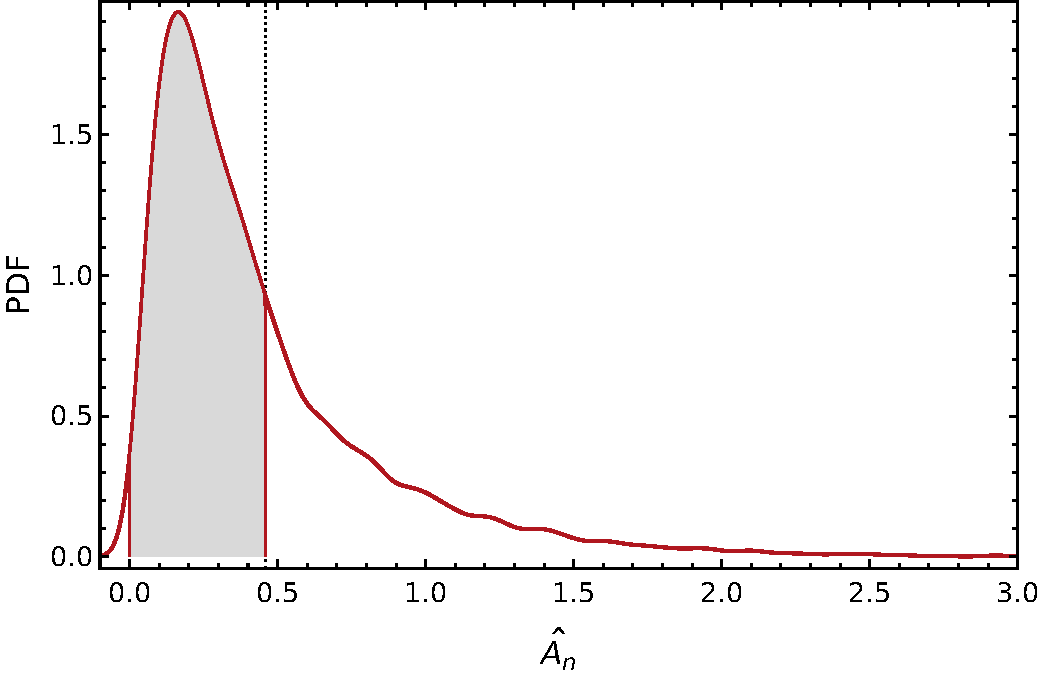
\includegraphics[width=9cm]{img/ad_dist}
\end{center}
\caption{Distribution of $\hat{A_n}$ generated from $10000$ replicas of a sample with $\hat{p} = 0.502994$. The area under the curve ranging from $[0,\hat{p}]$ is the $\pi$-value that represents the probability of measuring a value as extreme as $\hat{p}$. The measured $\pi$-value for this sample is $0.609$.}
\label{fig:ad_dist}
\end{figure}


\end{appendices}


\section*{Acknowledgements}
This work was supported by Conacyt-Mexico and MAE-Italy under grant 146498. We also thank Conacyt-Mexico for the support under  project grant 155492, Universidad Veracruzana under project 41504 and PRIN 2009 Italian grant ``Finitary and non-finitary probabilistic methods in Economics''. A segment of the IPC daily data set from 1978 to 2006 was provided by P. Zorrilla-Velasco, A. Reynoso del Valle and S. Herrera-Montiel, from BMV at that time. We are grateful to all of them.

\section*{References}
\begin{thebibliography}{15}

\bibitem{Anderson}
Bracquemond C, Cr\'etois E and Gaudoin O 2002 `A comparative study of goodness-of-fit tests for the geometric distribution and application to discrete time reliability' {\it Preprint} http://www-ljk.imag.fr/SMS/preprints.html.

\bibitem{monkeys}
Chen M K, Lakshminarayanan V and Santos L R 2006 `How Basic Are Behavioral Biases? Evidence from Capuchin Monkey Trading Behavior' {\it J. Political Econ.} {\bf 144} 517--537

\bibitem{Rama}
Cont R 2001 Empirical properties of asset returns: stylized facts and statistical issues' {\it Quantitative Finance} {\bf 1} 223--236

\bibitem{Achach}
Coronel-Brizio H F, Hern\'andez-Montoya A R, Huerta-Quintanilla R, and Rodr\'{\i}guez-Achach M E 2007 `Evidence of increment of efficiency of the Mexican Stock Market through the analysis of its variations', \textit{Physica A} (380) 391–398

\bibitem{Hernandez}
Hern\'andez Montoya A R, Coronel-Brizio H F, Rodr\'{\i}guez-Achach M E, Stevens-Ram\'{\i}rez G A, Politi M, and Scalas E 2011 `Emerging properties of financial time series in the Game of Life' {\it Phys. Rev.} E {\bf 84} 066104

\bibitem{leroy}
Leroy S F 1973, `Risk aversion and the martingale property of stock prices' {\it International Economic Review} {\bf 14} 436--446.

\bibitem{lucas} Lucas R E 1978, `Asset prices in an exchange economy'  {\it Econometrica} {\bf 46} 1429--1445.

\bibitem{lo} 
Lo A W and Mackinlay A C 1999, {\it A Non-Random Walk Down Wall Street}, (Princeton: Princeton University Press).

\bibitem{scalasold} Scalas E 1998, `Scaling in the market of futures', {\it Physica} A {\bf 253} 394--402.

\bibitem{French}
Mba.tuck.dartmouth.edu. (2015). Kenneth R. French - Data Library. [online] Available at: http://mba.tuck.dartmouth.edu/pages/faculty/ken.french/data\_library.html [Accessed 11 Oct. 2019].

\bibitem{Holyst}
Ho\l{yst} J A and Sieczka P 2008 `Statistical properties of short term price trends in high frequency stock market data' {\it Physica} A {\bf 387} 1218--1224

\bibitem{inpc}
Instituto Nacional de Estad\'istica, Geogrf\'ia e Inform\'atica. \'Indice Nacional de Precios al Consumidor. (2011, 5 de noviembre). http://www.inegi.org.mx/est/contenidos/proyectos/inp/inpc.aspx.

\bibitem{gainloss}
Jensen M H, Johansen A and Simonsen I 2002 `Inverse Statistics in Economic: The gain-loss asymmetry', {\it Physica} A {\bf 324} 6.

\bibitem{Levy-Solomon}
Levy M, Levy H and Solomon S 2000 {\it Microsimulations of Financial Markets: From Investor Behavior to Market Phenomena} (London: Academic Press)

\bibitem{Mantegna}
Mantegna R N and Stanley H E 2000 {\it An Introduction to Econophysics}. (Cambridge: University Press)

\bibitem{Lux}
Samanidou E, Zschischang E, Stauffer D and Lux T 2006 `Microscopic Models of Financial Markets'. Economics Working Paper 2006-15. Department of Economics, University of Kiel.

\bibitem{Samuelson 2}
Samuelson P A 1965 ‘Proof that Properly Anticipated Prices Fluctuate Randomly’, {\it Industrial Management Rev.} {\bf 6} 41--45.

\bibitem{Samuelson}
Samuelson P A and Nordhaus W D 2005 {\it Economics} (New York: McGraw-Hill)

\bibitem{NYSE}
Totha B and Kerteszb J `Increasing market efficiency: Evolution of cross-correlations of stock returns' {\it Physica} A {\bf 320} 505--515

\bibitem{cpi}
U. S. Bureau of Labor Statistics, Consumer Price Index. [Accessed 5 Nov. 2011]. http://data.bls.gov/timeseries/CUSR0000SA0?output\_view=pct\_1mth.

\bibitem{Voit}
Voit J 2003 {\it The Statistical Mechanics of Financial Market}. (New York: Springer-Verlag)

\bibitem{BraCreGau}
Bracquemond, C., Cr\'{e}tois, E., Gaudoin O., (2002)
``A comparative study of goodness-of-fit tests for the geometric distribution and application
to discrete-time reliability'' Technical Report, URL: www-ljk.imag.fr/SMS/ftp/BraCreGau02.pdf.

\bibitem{Choulakian}
Choulakian, V., Lockhart, R. A., Stephens, M. A., (1994)
% ``Cramer-von Mises Statistics for Discrete Distributions''
{\it The Canadian Journal of Statistics}, 22, 1, pp. 125-137. 

\bibitem{Nikulin}
Nikulin, M. S. (1992),
% ``Gihman statistics and Goodness-of-Fit Tests for Grouped Data''
{\it C. R. Math. Rep. Acad. Sci. Canada}, 14, 4, pp. 151-156.

\end{thebibliography}

\end{document}

